\section{Bài tập chuyên đề}

\subsection{Củng cố}

\begin{tuluyen}
Chọn phát biểu đúng về lipid và chất béo:
\begin{tasks}(2)
\task Mọi lipid đều là chất béo.
\task Chất béo là triester của glycerol và acid béo.
\task Chất béo tan tốt trong nước.
\task Chất béo chỉ có ở động vật.
\end{tasks}
\dapso{B.}
\end{tuluyen}

\begin{tuluyen}
Viết công thức tổng quát của chất béo đơn giản. Cho biết các nguyên liệu tạo nên một phân tử chất béo.
\dapso{\ce{(RCOO)3C3H5}; glycerol và ba acid béo.}
\end{tuluyen}

\begin{tuluyen}
Viết phương trình hóa học của các phản ứng:
\begin{tasks}(2)
\task Chất béo tác dụng với \ce{NaOH}, đun nóng.
\task Acid béo \ce{RCOOH} tác dụng với \ce{NaOH}.
\task Glucose tham gia phản ứng tráng bạc.
\task Glucose lên men tạo ethylic alcohol.
\task Saccharose bị thủy phân.
\task Tinh bột bị thủy phân hoàn toàn.
\task Cellulose bị thủy phân hoàn toàn.
\end{tasks}
\dapso{Xem các phương trình trong phần lí thuyết.}
\end{tuluyen}

\begin{tuluyen}
Nêu hiện tượng khi nhỏ dung dịch iodine vào:
\begin{tasks}(2)
\task Hồ tinh bột.
\task Dung dịch glucose.
\task Dung dịch saccharose.
\task Sợi cellulose.
\end{tasks}
\dapso{Hồ tinh bột chuyển xanh tím; các mẫu còn lại không xuất hiện màu xanh tím đặc trưng.}
\end{tuluyen}

\begin{tuluyen}
Cho các tình huống sau: lòng trắng trứng được đun nóng; sữa bị kết tủa khi thêm acid; len lông cừu và tơ nylon được đốt với mẫu rất nhỏ. Hãy nêu hiện tượng có thể quan sát và giải thích dựa trên tính chất của protein.
\end{tuluyen}

\subsection{Luyện tập kĩ năng}

\begin{tuluyen}
Một mẫu chất béo tinh khiết có khối lượng \SI{89.0}{\gram}, được coi là tristearin \ce{(C17H35COO)3C3H5}. Mẫu chất béo phản ứng vừa đủ với dung dịch \ce{NaOH}, đun nóng. Tính khối lượng sodium stearate \ce{C17H35COONa} thu được. Cho $M_{\ce{(C17H35COO)3C3H5}}=890$ g/mol và $M_{\ce{C17H35COONa}}=306$ g/mol.
\dapso{\SI{91.8}{\gram}.}
\begin{loigiaiBT}
\[
n_{\ce{(C17H35COO)3C3H5}}=\frac{89.0}{890}=\SI{0.100}{\mole}.
\]
\bangmol{7}
{\ce{(C17H35COO)3C3H5} & + & \ce{3NaOH} & \rightarrow & \ce{3C17H35COONa} & + & \ce{C3H5(OH)3}}
{0.100 & & & & 0.300 & &}
\[
m_{\ce{C17H35COONa}}=0.300\times306=\SI{91.8}{\gram}.
\]
\textbf{Vậy,} thu được \SI{91.8}{\gram} sodium stearate.
\end{loigiaiBT}
\end{tuluyen}

\begin{tuluyen}
Thủy phân hoàn toàn \SI{81.0}{\gram} tinh bột, hiệu suất quá trình đạt $80\%$. Tính khối lượng glucose thực tế thu được. Cho $M_{\ce{(C6H10O5)}}=162$ g/mol và $M_{\ce{C6H12O6}}=180$ g/mol.
\dapso{\SI{72.0}{\gram}.}
\begin{loigiaiBT}
Sơ đồ phản ứng cho biết một mắt xích \ce{C6H10O5} tạo một phân tử glucose:
\[
n_{\ce{C6H10O5}}=\frac{81.0}{162}=\SI{0.500}{\mole}.
\]
\bangmol{5}
{\ce{C6H10O5} & + & \ce{H2O} & \rightarrow & \ce{C6H12O6}}
{0.500 & & & & 0.500}
\[
m_{\ce{C6H12O6},\text{lt}}=0.500\times180=\SI{90.0}{\gram}.
\]
\[
m_{\ce{C6H12O6}}=90.0\times0.80=\SI{72.0}{\gram}.
\]
\textbf{Vậy,} khối lượng glucose thực tế thu được là \SI{72.0}{\gram}.
\end{loigiaiBT}
\end{tuluyen}

\begin{tuluyen}
Một mẫu glucose có khối lượng \SI{18.0}{\gram} tham gia phản ứng tráng bạc với hiệu suất $90\%$. Tính khối lượng bạc thu được. Cho $M_{\ce{C6H12O6}}=180$ g/mol và $M_{\ce{Ag}}=108$ g/mol.
\dapso{\SI{19.44}{\gram}.}
\begin{loigiaiBT}
\[
n_{\ce{C6H12O6}}=\frac{18.0}{180}=\SI{0.100}{\mole}.
\]
\bangmol{7}
{\ce{C6H12O6} & + & \ce{Ag2O} & \rightarrow & \ce{C6H12O7} & + & \ce{2Ag}}
{0.100 & & & & & & 0.200}
\[
m_{\ce{Ag},\text{lt}}=0.200\times108=\SI{21.6}{\gram}.
\]
\[
m_{\ce{Ag}}=21.6\times0.90=\SI{19.44}{\gram}.
\]
\textbf{Vậy,} khối lượng bạc thu được là \SI{19.44}{\gram}.
\end{loigiaiBT}
\end{tuluyen}

\subsection{Bài tập mục tiêu}

Các bài sau được trích nguyên văn từ đề tuyển sinh trong kho đề. Đây là những nhiệm vụ học sinh cần làm được sau khi hoàn thành chuyên đề. Một số dữ kiện nâng cao được giữ nguyên theo đề; kiến thức mở rộng cần thiết đã được nêu ngay trong câu hỏi.

\begin{tuluyen}
So sánh thành phần nguyên tố, cấu tạo và tính chất vật lí đặc trưng của dầu, mỡ dùng làm thực phẩm với dầu, mỡ dùng để bôi trơn xe, máy (được tách ra từ dầu mỏ). Trình bày phương pháp hóa học phân biệt hai loại chất trên.

Sự cố tràn dầu trên sông, biển gây thiệt hại rất lớn về kinh tế và môi trường. Để thu hồi dầu tràn người ta dùng hệ thống phao để gom dầu tràn vào một khu vực, sau đó hút vào các bồn lớn trên tàu. Để thu được dầu, người ta ly tâm để tách dầu khỏi hỗn hợp lỏng thành lớp nước ở dưới và dầu ở trên. Mở van xả để loại bỏ nước phía dưới, thu được lớp dầu.
\begin{enumerate}
\item Hãy cho biết 2 tác hại về môi trường khi xảy ra sự cố tràn dầu trên sông, biển?
\item Hãy cho biết quá trình ly tâm để tách hỗn hợp lỏng dựa trên các cơ sở nào?
\end{enumerate}
\source{Trích nguyên văn Câu 1, đề tuyển sinh lớp 10 chuyên Hóa Thái Nguyên 2026.}
\dapso{Chất béo thực phẩm là triglyceride, chứa C, H, O; dầu bôi trơn chủ yếu là hydrocarbon. Có thể phân biệt bằng phản ứng xà phòng hóa với \ce{NaOH}, đun nóng. Dầu tràn có thể hạn chế sự hòa tan oxygen và gây hại sinh vật; ly tâm dựa trên sự không tan lẫn và sự khác nhau về khối lượng riêng.}
\end{tuluyen}

\begin{tuluyen}
Nhà máy X sử dụng nguyên liệu mỡ động vật để sản xuất xà phòng. Thành phần của loại mỡ này chứa 80\% khối lượng là \ce{(C17H35COO)3C3H5}, còn lại là các tạp chất trơ và không có acid béo tự do. Để sản xuất 4000 bánh xà phòng (mỗi bánh có khối lượng 90 gam có chứa 76,5\% khối lượng muối \ce{C17H35COONa}), nhà máy X cần sử dụng $m$ kg loại mỡ trên cho phản ứng xà phòng hóa với dung dịch \ce{NaOH}. Biết hiệu suất của toàn bộ quá trình là 90\%. Tính giá trị của $m$.
\source{Trích nguyên văn Câu 6, đề tuyển sinh chuyên Hóa Cần Thơ 2026.}
\dapso{$m\approx\SI{370.83}{\kilo\gram}$.}
\begin{loigiaiBT}
Khối lượng sodium stearate cần thu:
\[
m_{\ce{C17H35COONa}}=4000\times90\times0.765=\SI{275400}{\gram}.
\]
\bangmol{7}
{\ce{(C17H35COO)3C3H5} & + & \ce{3NaOH} & \rightarrow & \ce{3C17H35COONa} & + & \ce{C3H5(OH)3}}
{x & & & & 3x & &}
\[
m_{\text{triglyceride,lt}}=275.4\times\frac{890}{3\times306}
=\SI{267.0}{\kilo\gram}.
\]
Khối lượng triglyceride có trong lượng mỡ thương mại cần dùng:
\[
m_{\text{triglyceride}}=\frac{267.0}{0.90}\approx\SI{296.67}{\kilo\gram}.
\]
Do mỡ chứa $80\%$ triglyceride:
\[
m=\frac{296.67}{0.80}\approx\SI{370.83}{\kilo\gram}.
\]
\textbf{Vậy,} cần khoảng \SI{370.7}{\kilo\gram} mỡ động vật.
\end{loigiaiBT}
\end{tuluyen}

\begin{tuluyen}
Trong công nghiệp, chất béo chủ yếu được sử dụng để điều chế glycerol, xà phòng và các loại sữa tắm. Để đánh giá chất lượng của chất béo dùng làm nguyên liệu sản xuất xà phòng, người ta sử dụng các chỉ số về chất béo như: chỉ số acid, chỉ số ester hóa.

Chỉ số acid là số mg \ce{KOH} cần dùng để phản ứng vừa đủ với acid béo tự do có trong 1 gam chất béo. Chỉ số ester hóa là số mg \ce{KOH} cần dùng để phản ứng vừa đủ với lượng triglyceride có trong 1 gam chất béo.

Một loại chất béo chỉ chứa các acid béo \ce{RCOOH} và triglyceride \ce{(RCOO)3C3H5}, trong đó \ce{R} là gốc hydrocarbon của các acid béo. Chất béo này có chỉ số acid là 7 và chỉ số ester hóa là 190,4. Cho 100 kg chất béo trên phản ứng hoàn toàn với dung dịch \ce{NaOH}, thu được $m$ kg muối \ce{RCOONa}. Toàn bộ lượng muối thu được, sau khi thêm tẩy màu rồi cho thêm phụ gia, chất tạo màu, hương liệu, được ép trong khuôn thành $x$ bánh xà phòng. Biết mỗi bánh xà phòng đều nặng 90 gam có chứa 80\% \ce{RCOONa} về khối lượng.
\begin{enumerate}
\item Viết các phương trình hóa học của các phản ứng xảy ra.
\item Tính giá trị của $x$.
\end{enumerate}
\source{Trích nguyên văn Câu 5.2, đề tuyển sinh lớp 10 chuyên Hóa Phú Thọ 2026.}
\dapso{Có khoảng 1436 bánh xà phòng đủ khối lượng.}
\begin{loigiaiBT}
Với \SI{100}{\kilo\gram} chất béo:
\[
n_{\ce{KOH, acid}}=\frac{7\times100\times10^3}{56\times10^3}=\SI{12.5}{\mole},
\qquad
n_{\ce{KOH, ester}}=\frac{190.4\times100\times10^3}{56\times10^3}=\SI{340}{\mole}.
\]
Khi thay \ce{KOH} bằng \ce{NaOH}, số mol kiềm phản ứng tương ứng không đổi.

\[
\ce{RCOOH + NaOH -> RCOONa + H2O}
\]
\[
\ce{(RCOO)3C3H5 + 3NaOH -> 3RCOONa + C3H5(OH)3}
\]
Số mol \ce{NaOH} tổng cộng là $12.5+340=\SI{352.5}{\mole}$, nên:
\[
m_{\ce{NaOH}}=352.5\times40=\SI{14100}{\gram}.
\]
Từ chỉ số ester hóa, số mol glycerol tạo thành:
\[
n_{\ce{C3H5(OH)3}}=\frac{340}{3}=\SI{113.333}{\mole}.
\]
Khối lượng nước tạo thành từ phản ứng acid béo:
\[
m_{\ce{H2O}}=12.5\times18=\SI{225}{\gram}.
\]
Khối lượng muối thu được:
\[
m_{\ce{RCOONa}}=100000+14100-225-113.333\times92
\approx\SI{103448.3}{\gram}.
\]
Mỗi bánh xà phòng chứa:
\[
m_{\ce{RCOONa, 1\ bánh}}=90\times0.80=\SI{72}{\gram}.
\]
\[
x=\frac{103448.3}{72}\approx1436.78.
\]
\textbf{Vậy,} có thể ép được tối đa 1436 bánh xà phòng đủ khối lượng quy định.
\end{loigiaiBT}
\end{tuluyen}

\begin{tuluyen}
Rơm rạ chiếm tỉ lệ lớn trong các phụ phẩm nông nghiệp ở Việt Nam. Với thành phần chứa hơn 40\% là chất X, rơm rạ là nguồn nguyên liệu thích hợp cho quá trình sản xuất ethanol. Quá trình này có thể được biểu diễn bằng sơ đồ sau:
\[
\ce{X ->[+H2O,\ H+,\ t] Y ->[xt] C2H5OH}.
\]
Trong sơ đồ trên, X và Y lần lượt là
\begin{tasks}(2)
\task tinh bột và glucose.
\task cellulose và fructose.
\task cellulose và glucose.
\task tinh bột và fructose.
\end{tasks}
\source{Trích nguyên văn Câu 16, đề tuyển sinh chuyên Hóa Lâm Đồng 2026.}
\dapso{C.}
\end{tuluyen}

\begin{tuluyen}
Khi nghiên cứu tốc độ phản ứng lên men glucose tạo thành ethylic alcohol với xúc tác là một loại enzyme, thu được kết quả và biểu diễn thành đồ thị như sau:

\begin{center}
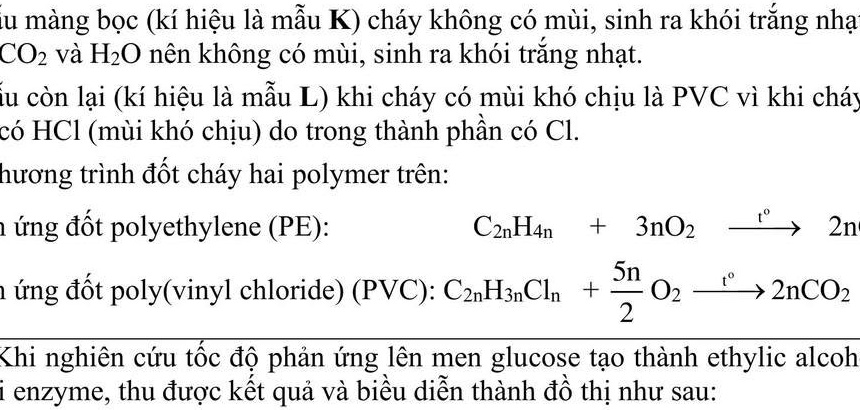
\includegraphics[width=0.72\textwidth]{data/assets/nb2026_lenmen_graph.jpg}
\end{center}

Nồng độ các chất trong đồ thị tính theo khối lượng chất tan (đơn vị gam) chất tan/thể tích dung dịch (đơn vị L). Giả thiết thể tích dung dịch không đổi trong quá trình thí nghiệm.
\begin{enumerate}
\item Viết phương trình phản ứng lên men trên.
\item Trong các khoảng thời gian 0 -- 12h, 12 -- 24h, 24 -- 36h, 36 -- 48h và 48 -- 60h, khoảng thời gian nào tốc độ chuyển hóa glucose là lớn nhất (không cần giải thích)?
\item Tính tốc độ chuyển hóa trung bình của glucose trong khoảng thời gian từ 0 h đến 60 h (theo đơn vị $\mathrm{g/(L.h)}$).
\item Tính hiệu suất quá trình lên men khi nồng độ ethylic alcohol sinh ra lớn nhất.
\end{enumerate}
\source{Trích nguyên văn Câu 5.2, đề tuyển sinh chuyên Hóa Ninh Bình 2026.}
\dapso{\ce{C6H12O6 -> 2C2H5OH + 2CO2}; 36--48 h; khoảng $0{,}67\,\mathrm{g/(L.h)}$; khoảng $87{,}07\%$.}
\end{tuluyen}
